\subsection{Estrutura do trabalho} \label{subsec:estrutura}



O trabalho está estruturado em diferentes capítulos, cada um abordando aspectos específicos da pesquisa. 
O Capítulo~\ref{sec:int}, Introdução, apresenta a introdução do trabalho, fornecendo uma contextualização do estudo, destacando a motivação e os objetivos a serem alcançados. Também são apresentados o problema em questão, a metodologia utilizada, a justificativa da pesquisa, as contribuições esperadas e a organização do trabalho.

O Capítulo~\ref{sec:refteo}, Revisão Teórica, oferece uma visão geral das principais pesquisas e estudos relacionados às questões abordadas na pesquisa. Esse capítulo proporciona uma base teórica sólida para fundamentar a análise e interpretação dos resultados.

No Capítulo~\ref{sec:base}, são apresentados os modelos que serão utilizados para trabalhar com os dados coletados. Essa seção detalha os modelos escolhidos, destacando suas características e fundamentos teóricos. Além disso, é realizado o detalhamento do estudo de caso utilizado na dissertação.

O Capítulo~\ref{sec:result}, Resultados, apresenta os resultados obtidos ao longo da pesquisa. Nesta seção, são realizadas análises e interpretações dos resultados, fornecendo insights relevantes para o entendimento do problema em estudo. Os resultados do estudo de caso são detalhados, evidenciando as principais descobertas e conclusões obtidas.

Por fim, o Capítulo~\ref{sec:conclusoes}, Conclusões, traz as considerações finais da pesquisa, abordando os principais achados e conclusões alcançadas. Também são apresentadas propostas para pesquisas futuras, visando expandir e aprofundar o conhecimento na área.

Essa estrutura organizada em capítulos permite uma apresentação clara e coerente do trabalho, abrangendo desde a introdução e fundamentação teórica até os resultados e conclusões finais.

 Este documento está estruturado em~\ref{sec:conclusoes} capítulos, divididos da seguinte forma:

\begin{figure}[H]
	\centering
	\caption{Estrutura da dissertação}
	\label{fig:estrutura}
	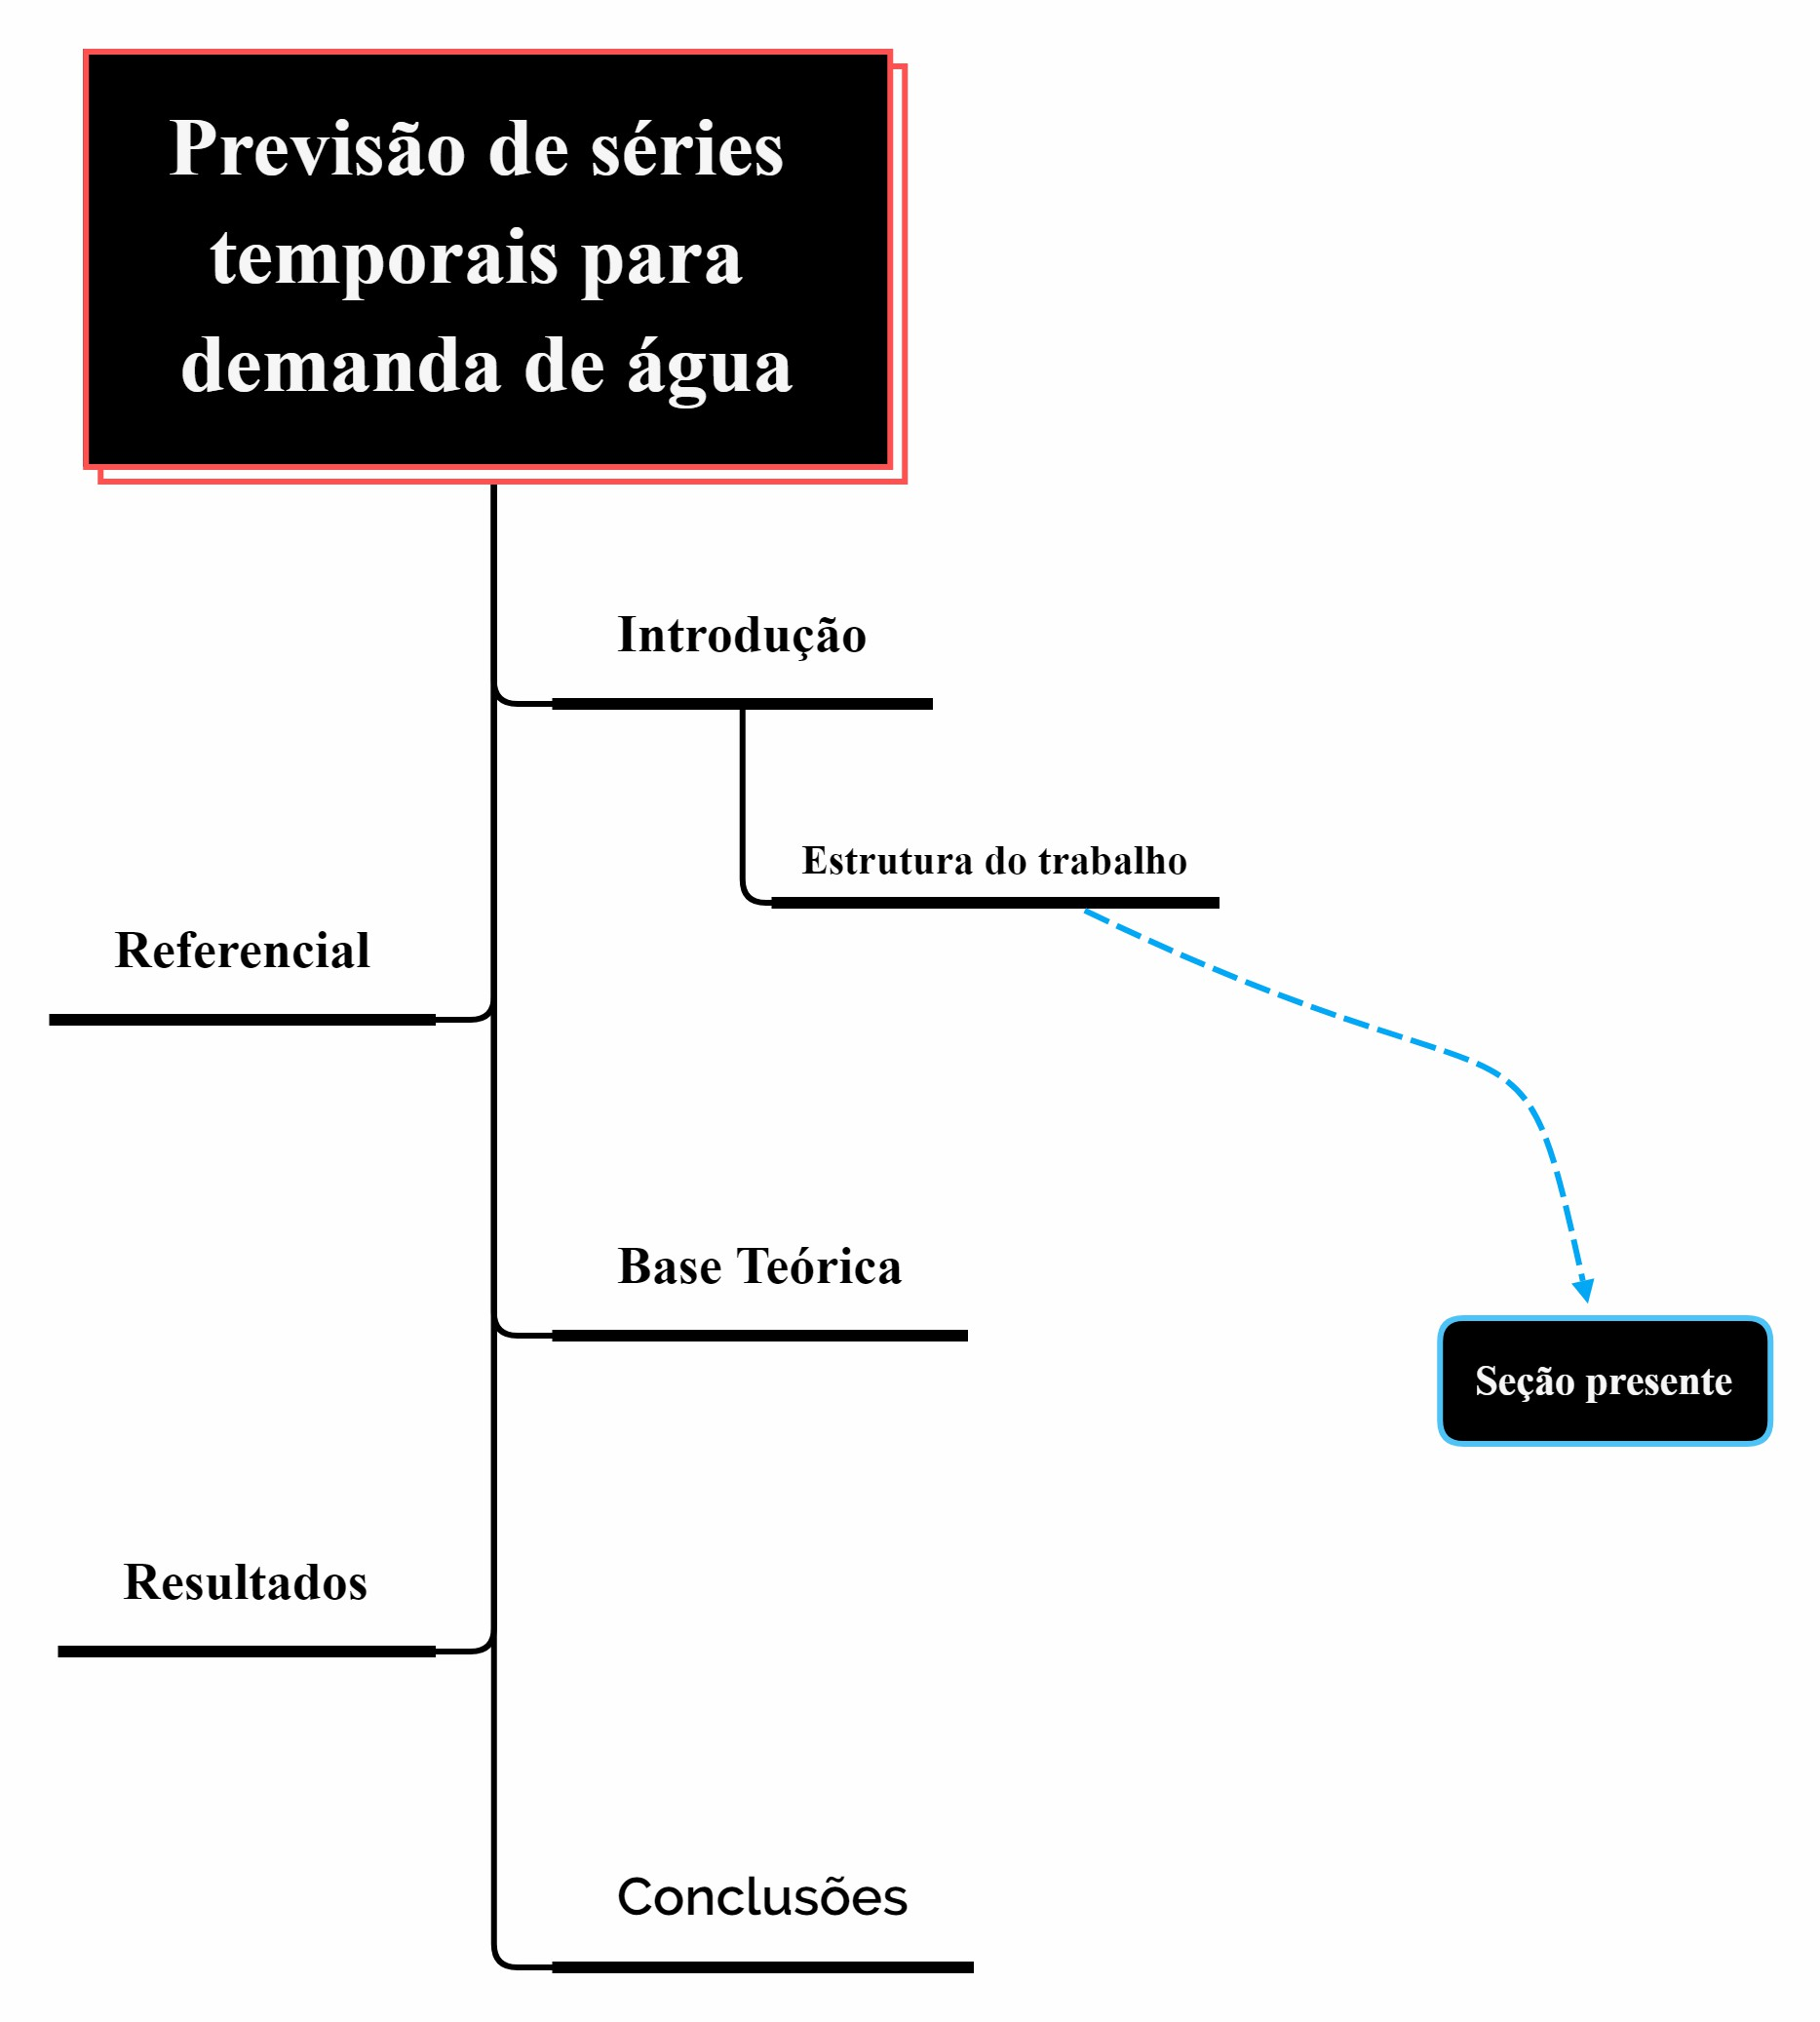
\includegraphics[width=0.9\linewidth]{Introducao/Figuras/Estrutura}
	
	Fonte: Elaboração própria 
\end{figure}
